\section{YOLOv1}  \label{sec:yolov1}

The first YOLO model was proposed in the "You Only Look Once: Unified, Real-Time Object Detection" paper in 2015 \cite{yolov1_2016}. Since there will be improved versions of the model, we denote this first model as YOLOv1, which is widely accepted in the computer vision research community \cite{understand_cnn_vs_yolo}. The YOLOv1 is designed to be a real-time object detection model. The YOLOv1 model is a three steps process, as shown in Figure \ref{fig:yolov1_process}. In the first step, the model takes an image of any size as input and resizes the image to the fixed size of $448 \times 448$. In the second step, the model predicts multiple bounding boxes, each box with a confidence (objectiveness) score, and multiple classifications for each detected object. Since the model predicts multiple bounding boxes and labels for each detected object, a non-maximum suppression (NMS) algorithm, as described in Subsection \ref{subsec:rpn}, is applied to assign one bounding box and one classification label per predicted object in the last step.

\begin{figure}[!ht]
    \centering
    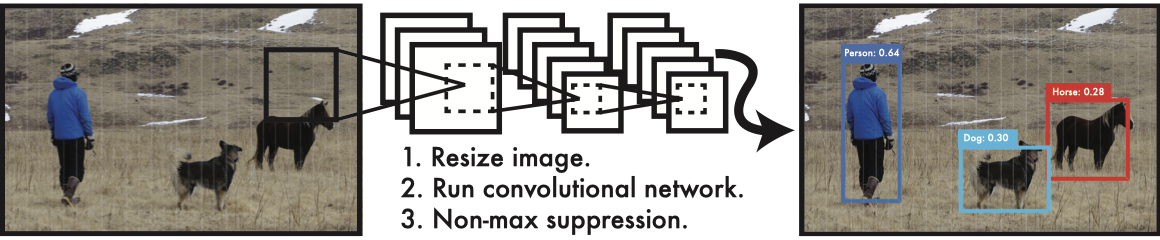
\includegraphics[width=4in]{figures/yolov1_process.png}
    \caption{YOLOv1 object detection process \cite{yolov1_2016}} 
    \label{fig:yolov1_process}
\end{figure}

In the original paper, the authors claim that the YOLOv1 model has three main benefits \cite{yolov1_2016}. First, YOLOv1 is extremely fast, processing 45 images per second compared to 7 images per second achieved by the Faster R-CNN model with VGG16 backbone. However, this is achieved at the cost of a 9.8\% reduction in mean average precision (mAP) score, i.e., 63.4\% and 73.2\% for the mAP score of YOLOv1 and Faster R-CNN, respectively. The second benefit is YOLOv1 learn a general representation of the object; thus, it tends to perform better compared to R-CNN based model when predicting for other domain like artwork. The third benefit is it sees the entire image during bounding box regression and classification compared to that of the R-CNN model, which only sees the RoI. This change allows YOLOv1 to encode contextual information about classes and thus reduce the number of false positives.

\subsection{Network Architecture}

\begin{figure}[!ht]
    \centering
    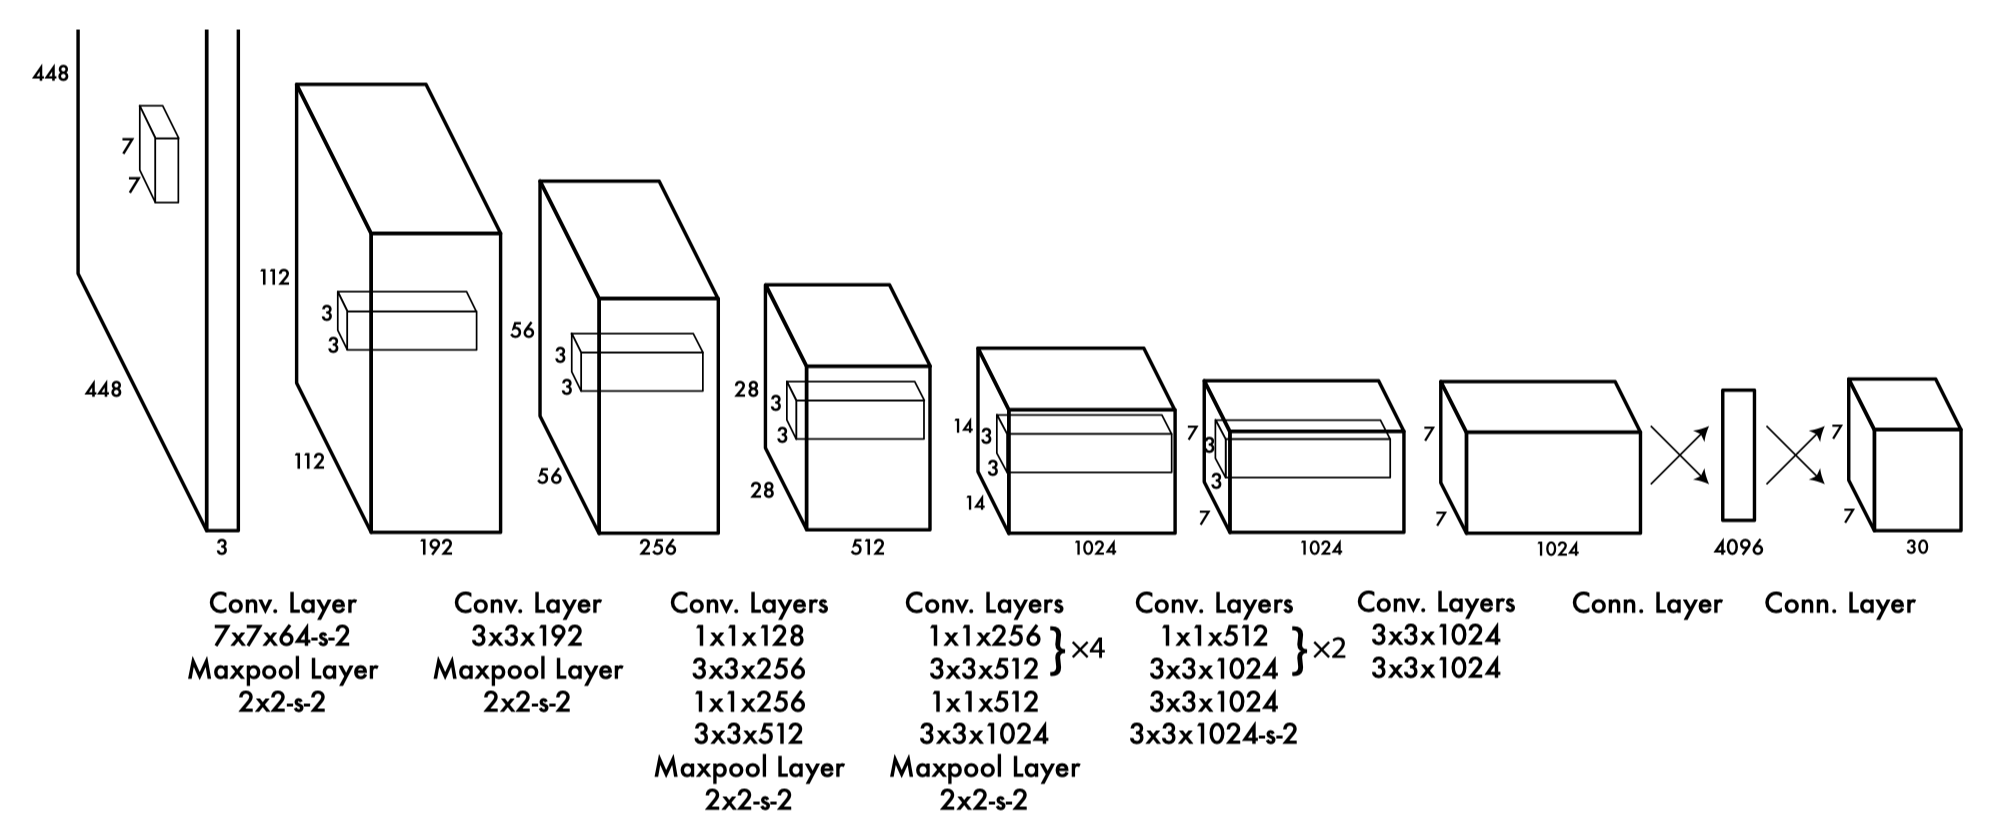
\includegraphics[width=4in]{figures/yolov1_archite.png}
    \caption{YOLOv1 architecture \cite{yolov1_2016}} 
    \label{fig:yolov1_archite}
\end{figure}

The YOLOv1 model is a convolutional neural network (CNN) based on the GoogLeNet model for image classification \cite{googlenet_2015}. The YOLOv1 model consists of 24 convolutional layers and end with 2 fully connected layer. The overall architecture of the YOLOv1 network is shown in Figure \ref{fig:yolov1_archite}. The author replaces the inception layers in GoogLeNet with $1 \times 1$ and $3 \times 3$ convolutional layer pair. All the layers in the YOLOv1 network, with the exception of the final layer, utilize the leaky ReLU activation function \cite{leaky_relu}, described as:
\begin{equation*}
    \phi(x) = 
    \begin{cases}
        x      & \text{if } x > 0 \\
        0.01 x & \text{otherwise}
    \end{cases}
\end{equation*}

As we can see in Figure \ref{fig:yolov1_archite}, the last convolutional layers in the network produce a feature map of size $7 \times 7 \times 1024$. This feature map is then processed by two fully connected layers. The last fully connected layer is responsible for predicting both the bounding box and the class label probability \cite{yolov1_2016}. This layer uses a linear activation function. The classification process in the last fully connected layer is similar to other CNN, where the layer is randomly initialized and can be optimized through training. On the other hand, YOLOv1 proposed a new bounding box regression method that is able to predict all bounding boxes of all objects present in the image at once, instead of processing each RoI individually one by one like the regressor implemented in Faster R-CNN. We will discuss this bounding box generation process in the next subsection.

\subsection{Bounding Box Generation}
To predict the bounding box, the YOLOv1 model divides the image into an $S \times S$ grid of equal cells. Each grid cell is then predicted $B$ bounding boxes and $C$ probabilities for the $C$ supported classes \cite{yolov1_2016}. The $S$ and $B$ values are hyperparameters and can be fine tune through the experiment. The $C$ value is the number of classes in the training dataset. In other words, $C=20$ if the training dataset is PASCAL VOC \cite{pascal_voc_2015} and $C=80$ if the training dataset is COCO dataset \cite{coco_2014}.

Each bounding box is represented by 5 values: coordinate $x$, coordinate $y$, width $w$, height $h$, and a confidence score. The $(x, y)$ coordinates are the center of the bounding box relative to a grid cell. The width $w$ and height $h$  is the dimension of the bounding box in 2D space. The value of $w$ and $h$ are normalized with respect to the input image width and height; thus, they are bounded by [0, 1]. The confidence score denotes the model's confidence in saying there is an object present in this cell, i.e., the objectiveness probability.

\begin{figure}[!ht]
    \centering
    \subfloat[][{YOLOv1 predict a bounding box for $cell_{32}$ with $S=3$ and $B=1$}]{ 
        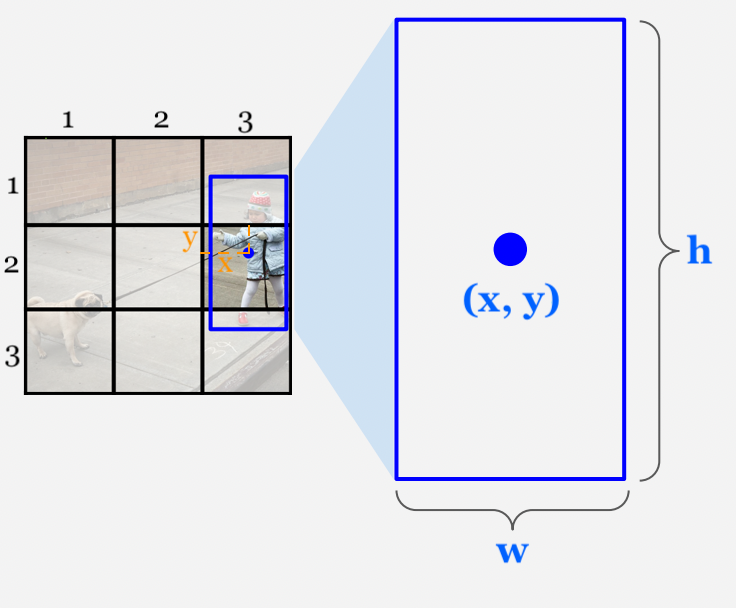
\includegraphics[height=2in]{figures/yolov1_bbox1.png} \label{fig:yolov1_bbox1}
    }
    \qquad \qquad
    \subfloat[][{YOLOv1 predict a bounding boxes for $cell_{32}$ with $S=3$ and $B=2$}]{ 
        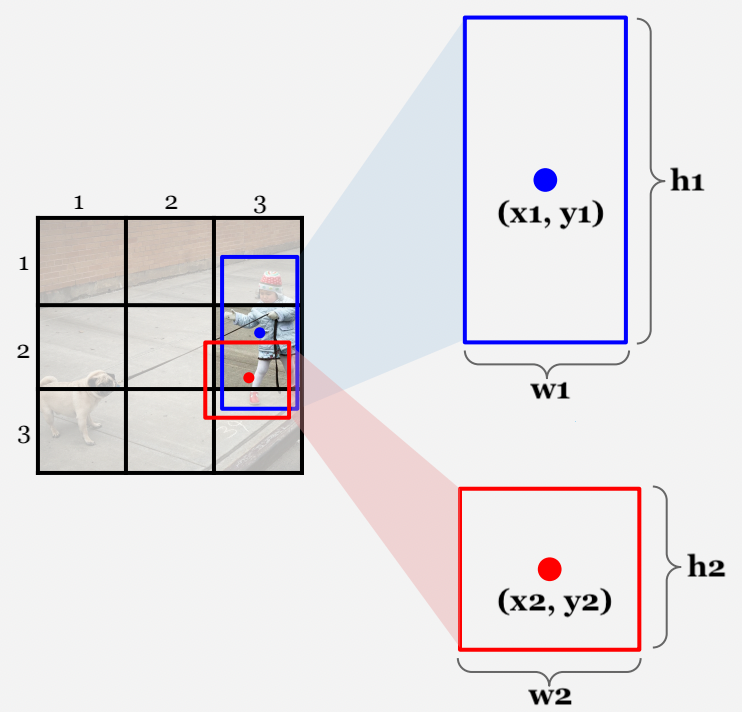
\includegraphics[height=2in]{figures/yolov1_bbox2.png} \label{fig:yolov1_bbox2}
    }
\end{figure}

As an example, consider processing an image with $S=3$, $B=1$, and classifying between two classes, human and dog ($C=2$), as demonstrated in Figure \ref{fig:yolov1_bbox1}. Since $B=1$, which means we only predict one bounding box per cell, then the cell$_{32}$ will return a tensor representing the predicted bounding box as:
\begin{equation*}cell
	cell's\ output = \begin{bmatrix}
        {\color{blue} x \quad y \quad w \quad h \quad conf} \quad p_{human} \quad p_{dog}
        \end{bmatrix}
\end{equation*}
where $conf$ is the confidence score, $p_{human}$ and $p_{dog}$ are the probability that the object belongs to the human and dog class, respectively. Noted that when we only predict 1 bounding box per cell, the YOLOv1 model predicts $(4+1+2)$ values for each cell, where 4 values describe the bounding box location, 1 for confidence score, and 2 probability values with one for each class. Therefore we say that when $B=1$, the model predicts $(4+1+C)$ for each cell. 

Now, we consider the example residing in Figure \ref{fig:yolov1_bbox2}, which is the same setup as the previous example but with $B=2$. In this second example, we predict two bounding boxes per cell, then the cell$_{32}$ return the following tensor for the two bounding boxes:
\begin{equation*}
    cell's\ output = \begin{bmatrix}
        {\color{blue} x_1 \quad y_1 \quad w_1 \quad h_1 \quad conf_1} \quad 
        {\color{red} x_2 \quad y_2 \quad w_2 \quad h_2 \quad conf_2} \quad 
        p_{human} \quad p_{dog} 
    \end{bmatrix}
\end{equation*}
The cell output a $(4+1)*2+C$ elements tensor when the model predicts two bounding boxes per cell. Therefore, we can generalize that the cell's prediction is encoded as $(4+1)*B+C$ tensor.

The computed prediction for each cell in the grid is stacked side by side and creates the depth for the image. That is, we divide a 2-dimensional image into a grid of $S \times S$ cells, and we predict a $(4+1)*B+C$ tensor for each cell; these predictions create the third dimension of the image. Therefore the prediction for the image is encoded as $S \times S \times [(4+1)*B+C]$ tensor. 

The YOLOv1 architecture shown in Figure \ref{fig:yolov1_archite} is for predicting 20 classes in PASCAL VOC with $S=7$ and $B=2$, thus the model predicting a $7 \times 7 \times 30$ tensor which encoded multiple bounding boxes and classification for each ground-truth object. 

\subsection{Training}
The first 20 convolutional layers of YOLOv1 are trained with the input size of $224 \times 224$ for the classification task on the ImageNet2012 dataset \cite{ImageNet_dataset}. Then 4 new convolutional layers and 2 fully connected layers are added. These new layers are randomly initialized. Additionally, the input size is increased to $448 \times 448$ for object detection task \cite{yolov1_2016}. With the initialized network, the model generates multiple bounding boxes and classifications, as described previously. While the YOLOv1 model applies NMS to choose which predicted bounding box to keep at inference time, the author used a different scheme to choose which predicted bounding box to contribute to the loss function. The scheme is choosing the predictor with the predicted box that has the highest IoU with a ground truth box. This lead to each predictor having a different specialization, which means each predictor is better at predicting a certain size, aspect ratio, or object's class \cite{yolov1_2016}.

The YOLOv1 model is trained to optimize for the sum-square error, which encodes both the bounding box coordinate loss and the classification loss \cite{yolov1_2016}. While the sum-square error allows easier optimization, it has some shortcomings and is not ideal if the model needs to optimize for average precision. The first critical shortcoming is it weighs the localization error and classification error equally \cite{yolov1_2016}. In an image, since the majority of the cells do not contain any object, which means the confidence score for these cells is 0, thus cause model always has a poor performance for the classification task. This also causes the bounding box error to have little effect on the total error. Thus a scalar term is added to the loss to weight the bounding box error higher than the classification error \cite{yolov1_2016}. The second critical shortcoming is the sum-squared error weight the offset in the large bounding box and small bounding box equally \cite{yolov1_2016}. This is not ideal since the total number of pixels in the large bounding box is larger than the smaller bounding box; thus, offsetting by certain pixels has a larger effect on the smaller bounding box than the larger bounding box. To partially resolve this, the YOLOv1 model performs the error calculation on the square root of the bounding box width and height instead of the width and height directly.